\documentclass[12pt, oneside]{article}  	% use "amsart" instead of "article" for AMSLaTeX format
\usepackage[margin=2.25cm]{geometry}        		% See geometry.pdf to learn the layout options. There are lots.
\geometry{letterpaper}          		% ... or a4paper or a5paper or ... 
%\geometry{landscape}        		% Activate for rotated page geometry
%\usepackage[parfill]{parskip}  		% Activate to begin paragraphs with an empty line rather than an indent
\usepackage{graphicx}				% Use pdf, png, jpg, or eps§ with pdflatex; use eps in DVI mode
								% TeX will automatically convert eps --> pdf in pdflatex	
								
%\usepackage[T1]{fontenc}
%\usepackage[utf8]{inputenc}
%\usepackage{babel}
%\usepackage{csquotes}
									
\usepackage{amssymb}
\usepackage{lineno}
\usepackage{setspace}
\doublespacing
\usepackage{authblk}
\usepackage{hyperref}
\usepackage{xcolor}

%\usepackage{pythonhighlight}

\usepackage[utf8]{inputenc}

% Default fixed font does not support bold face
\DeclareFixedFont{\ttb}{T1}{txtt}{bx}{n}{10} % for bold
\DeclareFixedFont{\ttm}{T1}{txtt}{m}{n}{10} % for normal

% Custom colors
\usepackage{color}
\definecolor{deepblue}{rgb}{0,0,0.5}
\definecolor{deepred}{rgb}{0.6,0,0}
\definecolor{deepgreen}{rgb}{0,0.5,0}

\usepackage{listings}

\newcommand\terminalstyle{\lstset{
basicstyle=\ttm,
frame=none,             % Any extra options here
aboveskip=20pt,
belowskip=20pt,
xleftmargin=0.5cm,
}}
\lstnewenvironment{terminal}[1][]
{
\terminalstyle
\lstset{#1}
}
{}


% Python style for highlighting
\newcommand\pythonstyle{\lstset{
language=Python,
basicstyle=\ttm,
morekeywords={self},       % Add keywords here
keywordstyle=\ttb\color{deepblue},
emph={MyClass,__init__},     % Custom highlighting
emphstyle=\ttb\color{deepred},  % Custom highlighting style
stringstyle=\color{deepgreen},
frame=none,             % Any extra options here
showstringspaces=false,
numbers=none,
numbersep=5pt,
aboveskip=20pt,
belowskip=20pt,
xleftmargin=0.5cm,
}}

% Python environment
\lstnewenvironment{python}[1][]
{
\pythonstyle
\lstset{#1}
}
{}

% Python for external files
\newcommand\pythonexternal[2][]{{
\pythonstyle
\lstinputlisting[#1]{#2}}}

% Python for inline
\newcommand\pythoninline[1]{{\pythonstyle\lstinline!#1!}}


\usepackage{natbib}
\setcitestyle{aysep={}} 

\usepackage{lipsum} 

\hypersetup{
  colorlinks,
  linkcolor={red!50!black},
  citecolor={blue!50!black},
  urlcolor={blue!80!black}
}

\author[1,*]{Joseph D. Hughes}
\affil[1]{\small U.S. Geological Survey, Integrated Modeling and Prediction Division, 927 W Belle Plaine Ave, Chicago, IL, USA}
\author[2]{Christian D. Langevin}
\affil{\small U.S. Geological Survey, Integrated Modeling and Prediction Division, 2280 Woodale Dr, Mounds View, MN, USA}
\author[3]{Scott R. Paulinski}
\affil[3]{\small U.S. Geological Survey, California Water Science Center, 3130 Skyway Drive, Suite 602, Santa Maria, CA, USA}
\author[4]{Joshua D. Larsen}
\affil[4]{\small U.S. Geological Survey, California Water Science Center, 6000 J Street, Placer Hall, Sacramento, CA, USA}
\author[5]{David Brakenhoff}
\affil[5]{\small Artesia Water, Korte Weistraat 12, Schoonhoven, Netherlands}
\affil[*]{\small Corresponding author jdhughes@usgs.gov}


\begin{document}

\onecolumn
\raggedright
\widowpenalty10000
\clubpenalty10000
\setlength\parindent{2em}

\title{Research Paper/ \\FloPy Workflows for Creating and Constructing Structured and Unstructured MODFLOW 6 Models} 

\maketitle


\begin{abstract}

\noindent FloPy is a Python package for creating, running, and post-processing MODFLOW-based groundwater flow and transport models. FloPy functionality has expanded to support the latest version of MODFLOW (MODFLOW 6) including support for unstructured grids. FloPy can simplify the process required to download MODFLOW-based and other executables for Linux, MacOS, and Windows operating systems. Expanded FloPy capabilities include (1) full support for structured and unstructured spatial discretizations; (2) geoprocessing of spatial features and raster data to develop model input for supported discretization types; (3) the addition of functionality to provide direct access to simulated output data; (4) extension of plotting capabilities to unstructured MODFLOW 6 discretization types; and (5) the ability to export model data to shapefiles, NetCDF, and VTK formats for processing, analysis, and visualization by other software products. Examples of using expanded FloPy capabilities are presented for a hypothetical watershed. An unstructured groundwater flow and transport model, with several advanced stress packages, is presented to demonstrate how FloPy can be used to develop complicated unstructured model datasets from original source data (shapefiles and rasters), post-process model results, and plot simulated results.

\end{abstract}

\section*{Introduction}

FloPy is a Python package for constructing, running, and post processing MODFLOW-based groundwater flow and transport models \citep{bakker2016scripting}. It is open-source and developed by a growing community of contributors. The combination of open-source programming languages (such as Python) with version control software (such as Git) allows the model construction process to be documented, reproducible, and easily inspected and used by others. This workflow has been recommended as one way to facilitate repeatable research and sharing of ideas \citep{fienen2016}. \cite{bakker2016scripting} describe the general approach for working with models within the Python environment and emphasize the reproducible nature of developing models through scripting.

FloPy has been used to pioneer new methods and analysis tools, such as deep learning approaches for improving groundwater model calibration \citep{sun2018, zhou2021}, regionalizing residence times using metamodeling \citep{starn2018}, applying iterative ensemble approaches for calibration and uncertainty quantification \citep{white2018ies}, and exploring alternative parameterization schemes for risk analysis \citep{knowling2019}. There are numerous examples of constructing MODFLOW models with FloPy to solve applied groundwater problems \citep{befus2017, vanengelen2018, ebeling2019, zipper2019, befus2020}. FloPy is also being used in other software and workflows to improve repeatability and robustness through automated model construction \citep{white2020toward, fienen2022risk, larsen2022rapid, leaf2022modflow}. FloPy is also used in GIS-based tools, such as FREEWAT \citep{freewat2018} and other cyberinfrastructures \citep{essawy2018} to export models into MODFLOW datasets. FloPy can also be used as the ``glue'' to help couple MODFLOW to other hydrological models \citep{burek2020} or, for example, to agent-based models designed to quantify the effects of decision makers on environmental behavior \citep{jaxarozen2019}. 

The U.S. Geological Survey uses FloPy to teach MODFLOW and groundwater modeling to early- and mid-career engineers and scientists. Other organizations also use FloPy to teach MODFLOW \citep[\textit{e.g.,}][]{auswat2023, hatari2023}. We routinely rely on FloPy to load and help identify problems in user model applications, and with the initial release of the MODFLOW 6 groundwater flow model \citep{modflow6gwf}, we started to rely on FloPy to help with development of the MODFLOW program. We write tests that rely on FloPy to construct and run models, and then read output. We then verify that the output is as expected, by using analytical solutions, other models, or results that have been confirmed to be correct.

The purpose of this paper is to highlight FloPy new functionality for creating and constructing structured and unstructured MODFLOW models. We provide examples that demonstrate these new capabilities, and reinforce the advantages of the modern scripting workflow for developing reproducible structured and unstructured MODFLOW groundwater flow and transport models that can be updated as new data become available. The examples also demonstrate workflows that develop different model grids for the same model domain. The important advances described here include (1) complete support for all models, packages, and options implemented in the core version of MODFLOW supported by the U.S. Geological Survey \citep{modflow6framework, modflow6gwf, modflow6xt3d, langevin2020hydraulic, morway2021use, modflow6gwt, modflow6csub, modflow6lkt}; (2) generalized support for models based on a structured grid consisting of layers, rows, and columns, and also for models based on unstructured grids; (3) implementation of new geoprocessing capabilities to rapidly populate models with data from a variety of input sources; (4) simplified access to model results; (5) plotting capabilities for map and cross-section views of model data; and (6) export capabilities for writing model data to a variety of output formats.


\section*{FloPy Support for MODFLOW 6}

The most recent version of MODFLOW (MODFLOW 6) is an object-oriented program and framework developed to provide a platform for supporting multiple models and multiple types of models within the same simulation \citep{modflow6framework}. These models can be independent of one another with no interaction, they can exchange coefficients and dependent variables (\textit{e.g.}, head), or they can be tightly coupled at the matrix level by adding them to the same numerical solution. Transfer of information between models is isolated to exchange objects, which allow models to be developed and used independently. Within this new framework, a regional-scale groundwater model may be coupled with multiple local-scale groundwater models. 

MODFLOW 6 currently includes the Groundwater Flow (GWF) Model and the Groundwater Transport (GWT) Model each with packages to represent surface water processes, groundwater extraction, external boundaries, mass sources and sinks, and mass sorption and reactions. GWF and GWT models can be developed using structured model grids consisting of layers, rows, and columns or they can be developed using more general unstructured grids using many of the concepts and numerical approaches available in MODFLOW-USG \citep{modflowusg}. MODFLOW 6 also includes advanced formulations to simulate three-dimensional anisotropy and dispersion \citep{modflow6xt3d}, coupled variable-density groundwater flow and transport \citep{langevin2020hydraulic}, and a water mover package to represent natural and managed hydrologic connections \citep{morway2021use}.

Development and testing of the MODFLOW 6 program relies heavily on tight integration with FloPy. A key component of this tight integration is the capability to quickly support new MODFLOW 6 models and packages with FloPy. Unlike the FloPy support for previous MODFLOW versions (\textit{e.g.}, MODFLOW-2005, MODFLOW-NWT, MODFLOW-USG, and SEAWAT), the FloPy Python classes for MODFLOW 6 are dynamically generated from simple text files, called ``definition files,'' that describe the input file structure. All MODFLOW 6 model input files are described using these definition files. This allows MODFLOW 6 developers to write tests for new models, packages, and functionality as they are developed. These definition files are used to programmatically generate the user input and output guide for MODFLOW 6. These same definition files are also used to generate FloPy classes, with documentation corresponding to input variable descriptions in the input and output guide. New functionality can be added by users to existing packages by modifying existing definition files. The existing definition files can also be used as a template for creating classes for new MODFLOW 6 models or packages.

\section*{Common Modeling Tasks}

The code snippets presented in this section that demonstrate how to create model grids, geoprocess data, process output, plot model data, and export model data are available as Jupyter notebooks \citep{Kluyver:2016aa} at the internet addresses indicated in the \nameref{sec:summary} section.

\subsection*{Getting MODFLOW and Other Related Executables}

FloPy for MODFLOW 6 relies on a number of helper classes, which wrap functionality available in pre-compiled external utility programs, to generate unstructured models and calculate water budgets on user-defined zones. These external utility programs (\textit{e.g.}, GRIDGEN, Triangle, ZONEBUDGET, etc.), MODFLOW 6, and other MODFLOW-related programs (\textit{e.g.}, MODPATH, MT3DMS, MT3D-USGS, SEAWAT, etc.) can be installed using

\begin{terminal}
get-modflow :flopy
\end{terminal}

\noindent in a terminal or at the command line after installing FloPy. The \texttt{get-modflow} command detects the operating system (Linux, MacOS, or Windows) and downloads the latest operating-system-specific release of MODFLOW and related programs from an \href{https://github.com/MODFLOW-USGS/executables}{Executables GitHub repository}. \texttt{get-modflow} can also download previous versions of MODFLOW 6 and the latest development version of MODFLOW 6 using instructions available on the \href{https://github.com/modflowpy/flopy/blob/develop/docs/get_modflow.md}{FloPy GitHub repository}.

\subsection*{Managing and Creating Model Grids}

FloPy was originally developed to support models that are based on a structured grid consisting of layers, rows, and columns. Recent support for unstructured grids in MODFLOW \citep{modflowusg, modflow6gwf} required revisions to the underlying approach for managing spatial discretization information in FloPy. Grid information is containerized into a single location and used throughout FloPy modeling tasks for geospatial processing, plotting, and exporting. Spatial discretization is now handled in FloPy through dedicated model grid classes. There is a \texttt{Grid} class, which serves as the base class for the \texttt{StructuredGrid}, \texttt{VertexGrid}, and \texttt{UnstructuredGrid} classes. Grid objects can be created by the user for preprocessing, and they are automatically generated and attached to a FloPy model object.

Structured MODFLOW grids can have constant row and column spacings, as shown in Figure \ref{fig:grids}A, or they can have variable row and column spacings to focus resolution around an area of interest, as shown in Figure \ref{fig:grids}B. The following Python code shows how to create a \texttt{StructuredGrid} object in FloPy. A \texttt{StructuredGrid} object can also be created from discretization data required when instantiating a MODFLOW 6 \texttt{DIS} object using \texttt{flopy.mf6.ModflowGwfdis()}. 

\begin{python}
>>> structured_grid = flopy.discretization.StructuredGrid(nlay=nlay, 
... delr=delr, delc=delc, xoff=0.0, yoff=0.0, angrot=0.0, top=top, botm=botm)
\end{python}


\begin{figure}[ht!]
	\begin{center}
		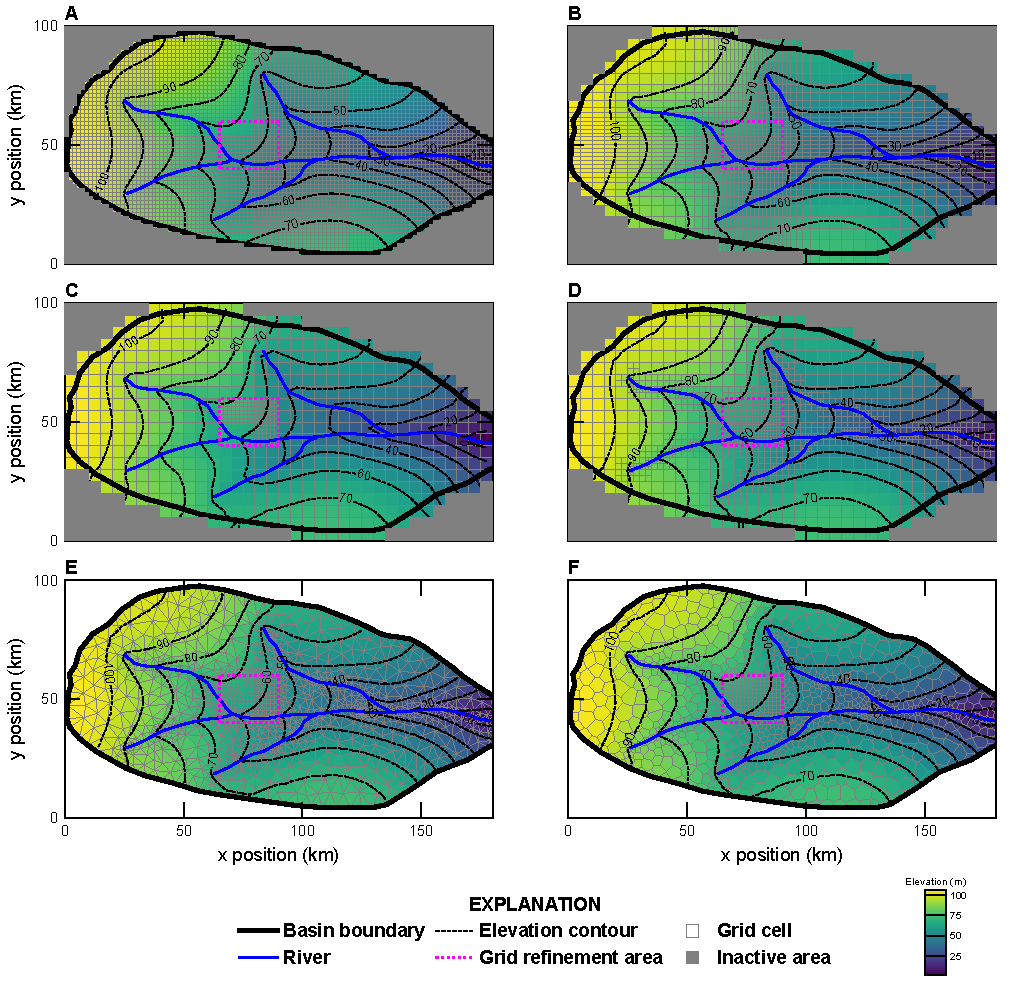
\includegraphics{figure1.pdf}
	\end{center}
	\caption{Examples of grids that can be generated and processed using FloPy for a hypothetical watershed, including (A) a structured MODFLOW grid with constant and equal row and column spacings, (B) a structured MODFLOW grid with variable row and column spacings, (C) a structured MODFLOW child grid nested within a structured MODFLOW parent grid, (D) a quadtree grid generated with the GRIDGEN program \citep{gridgen} through the FloPy wrapper, (E) a triangular grid generated with the Triangle program \citep{trianglemesh} through the FloPy wrapper, and (F) a Voronoi grid created from the triangular mesh. All of the grids have refinement in the location of the child grid in (C).}
	\label{fig:grids}
\end{figure}


MODFLOW 6 was developed to support multi-model simulations \citep{modflow6framework}. One form of multi-model simulation is a nested grid application in which a more finely discretized child model is embedded within a more coarsely discretized parent model \citep{modflowlgr, vilhelmsen2012evaluation, modflowlgr2, fienen2022simulation}. The use of a locally refined grid (LGR) within an encompassing parent grid offers computational benefits in that the additional refinement is targeted to an area of interest. FloPy provides a \texttt{Lgr()} utility class for constructing the data required to tightly couple parent and child models within a single MODFLOW 6 simulation. Figure \ref{fig:grids}C shows two \texttt{StructuredGrid} objects---one object represents the parent model grid and the other represents the nested child grid. The \texttt{Lgr()} utility class defines the connection properties between cells in the parent model and cells in the child model. Connection properties consist of distances, areas, and other geometric information needed to calculate flow between cells in different models. The \texttt{Lgr()} utility class is general in that the child model can have more layers than the parent model. The following Python code shows the steps for creating a child \texttt{StructuredGrid} object using data for the parent grid with the \texttt{Lgr()} utility class.

\begin{python}
idomain_parent = np.ones((nlay_parent, nrow_parent, ncol_parent), dtype=int)
idomain_parent[0, 8:12, 13:18] = 0
ncpp, ncppl = 3, [1]
lgr = Lgr(nlay_parent, nrow_parent, ncol_parent,
          delr_parent, delc_parent, topparent, botmparent,
          idomain_parent, ncpp=ncpp, ncppl=ncppl, 
          xllp=0.0, yllp=0.0)
delr, delc = lgr.get_delr_delc()
xoff, yoff = lgr.get_lower_left()
structured_gridchild = StructuredGrid(delr=delr, delc=delc,
                                      xoff=xoff, yoff=yoff)
\end{python}

\noindent The child grid is created in the inactive area of the parent grid (\texttt{idomain\_parent}) and the returned \texttt{lgr} object contains all of the information required to create a child \texttt{StructuredGrid} object. The connection properties needed to create the MODFLOW 6 Exchange input file for the parent and child grids can be retrieved using \texttt{lgr.get\_exchange\_data()}.

FloPy supports management and generation of unstructured grids. Unstructured grids are represented as layered or fully unstructured. A layered grid is one in which the same grid applies to all model layers. An unstructured grid is more general and allows the model grid to change with depth. Layered grids and unstructured grids are stored in FloPy as \texttt{VertexGrid} and \texttt{UnstructuredGrid} objects, respectively.

Layered quadtree grids can be created using the \texttt{Gridgen()} utility class, which is a wrapper around the GRIDGEN program \citep{gridgen}. GRIDGEN starts with a structured MODFLOW grid with constant and equal row and column spacing defined by the user. The program then recursively subdivides individual cells that intersect with refinement features into quarters until a maximum level of refinement is met. Refinement features may be points, lines, or polygons. Smoothing is automatically handled so that a cell is connected to no more than two cells in any primary horizontal direction and four cells in the vertical direction. Figure \ref{fig:grids}D shows an example of a quadtree grid created with GRIDGEN in which a base grid is refined two levels along streams and in the grid refinement area shown in Figure \ref{fig:grids}. The following Python code shows the steps for creating the quadtree grid with GRIDGEN.

\begin{python}
sim = flopy.mf6.MFSimulation()
gwf = flopy.mf6.ModflowGwf(sim)
dis6 = flopy.mf6.ModflowGwfdis(gwf, nrow=nrow, ncol=ncol, delr=dy, delc=dx)
g = Gridgen(dis6, model_ws=temp_path)
g.add_refinement_features([[lgr_polygon_xy]], "polygon", 2, range(1))
g.add_refinement_features(stream_points, "line", 2, range(1))
g.build(verbose=False)
gridprops_vg = g.get_gridprops_vertexgrid()
quadtree_grid = flopy.discretization.VertexGrid(**gridprops_vg)
\end{python}

FloPy also provides a wrapper utility for the Triangle mesh generation program \citep{trianglemesh}. The \texttt{Triangle()} utility class writes the Triangle program input file, runs the Triangle program, and then loads the triangular mesh. Users provide the maximum area for individual triangles, angle constraints, a polygon describing the model domain, and so forth. Figure \ref{fig:grids}E shows an example of a triangular grid created with the Triangle program. The Python code for creating the triangular grid is shown below.

\begin{python}
tri = flopy.utils.triangle.Triangle(maximum_area=maximum_area, 
                                    angle=30, nodes=refinement_verts,
                                    model_ws=temp_path)
tri.add_polygon(boundary_points)
tri.build(verbose=False)
cell2d = tri.get_cell2d()
vertices = tri.get_vertices()
triangular_grid = VertexGrid(vertices=vertices, cell2d=cell2d, 
                             idomain=idomain, nlay=nlay, ncpl=tri.ncpl, 
                             top=top, botm=botm)
\end{python}

\noindent \texttt{refinement\_verts} in the triangular grid code shown above contains the user-specified stream vertices and the horizontal cell vertices for the grid refinement area shown in Figure \ref{fig:grids}. 

A triangular grid can be converted by FloPy into a Voronoi grid using the \texttt{VoronoiGrid()} utility class. The \texttt{VoronoiGrid()} utility class uses SciPy routines \citep{2020SciPy-NMeth} to construct Voronoi polygons around each vertex in the triangular mesh. Figure \ref{fig:grids}F shows an example of a Voronoi grid created from the triangular mesh shown in Figure \ref{fig:grids}E. The steps for creating the Voronoi grid from the previously created \texttt{Triangle()} object (\texttt{tri}) are shown below.

\begin{python}
vor = flopy.utils.voronoi.VoronoiGrid(tri)
gridprops = vor.get_gridprops_vertexgrid()
voronoi_grid = VertexGrid(**gridprops, nlay=nlay, idomain=idomain)
\end{python}

The \texttt{StructuredGrid}, \texttt{VertexGrid}, and \texttt{UnstructuredGrid} classes have useful properties and methods for accessing or mapping locations on the model grid including: (1) converting x, y pairs from local to global coordinates (\texttt{.get\_coords()}) and from global to local coordinates (\texttt{.get\_local\_coords()}); (2) getting x, y, and z coordinates for cell centers (\texttt{.xcellcenters}, \texttt{.ycellcenters}, \texttt{.zcellcenters}, and \texttt{.xyzcellcenters}) and vertices (\texttt{.xvertices}, \texttt{.yvertices}, \texttt{.zvertices}, and \texttt{.xyzvertices}); and (3) intersecting a list of x, y pairs with the grid and returning the appropriate \texttt{cellid} (\texttt{.intersect()}). Local coordinates are model-based coordinates and global coordinates are coordinates generated after transforming local model coordinates using user-specified x-offset, y-offset, and rotation angle values; global coordinates are equal to local coordinates if the x-offset, y-offset, and rotation angle are all zero. Other useful grid class properties and methods include generating a grid object from a MODFLOW 6 binary grid file (\texttt{.from\_binary\_grid\_file()}), retrieving cell thicknesses (\texttt{.cell\_thickness}), and calculating the saturated thickness for each cell by passing a head array with dimensions consistent with the grid object (\texttt{.saturated\_thickness(head)}).

The new FloPy capabilities for generating and testing different types of model grids allows for innovation in the way a study area is discretized. For example, \cite{Moussa2018} used a Voronoi grid to add additional resolution in the vicinity of irrigation wells in the Frenchman Creek Basin in Nebraska, USA to quantify the effects of land-use change and irrigation on streamflow depletion. Furthermore, the ability to develop multi-model simulations using FloPy allows higher-resolution inset models to be added in focused areas. \cite{fienen2022simulation} used local grid refinement models tightly coupled to inset models that were in turn loosely coupled to a coarse regional model, to better represent lakes and quantify the effects of distant pumping on lake and groundwater interactions in the Central Sands region in Wisconsin, USA. The inset groundwater flow models with lakes \citep{fienen2022simulation} were developed using \texttt{modflow-setup} \citep{leaf2022modflow}, which relies on FloPy to generate MODFLOW 6 datasets.

\subsection*{Geospatial Processing}

Geospatial processing is often a fundamental part of creating a groundwater model. New geospatial processing functionality has been added to FloPy to help users construct models using data from common input sources. The geospatial processing functionality has been implemented to work with the different types of model grids so that it is straightforward to build and construct models with different grid resolutions or grid types. The geospatial processing routines work with all three of the model grid types (\texttt{StructuredGrid}, \texttt{VertexGrid}, and \texttt{UnstructuredGrid}). 

A common geospatial processing task is resampling of raster data onto a model grid. For example, it is often necessary as part of model construction to resample a raster data set of land surface elevation onto a model grid. FloPy includes a new raster sampling utility based on the Rasterio Python package \citep{gillies_2019}. The following Python code demonstrates the steps for resampling an Esri ASCII raster format grid onto a Voronoi grid.

\begin{python}
fine_topo = flopy.utils.Raster.load("./grid_data/fine_topo.asc")
top_vg = fine_topo.resample_to_grid(voronoi_grid, band=fine_topo.bands[0],
                                    method="linear", extrapolate_edges=True)
\end{python}

\noindent The result of raster resampling is a NumPy array, equal in size to the number of cells in one layer of the Voronoi grid. The NumPy array contains an interpolated land surface elevation for each model cell. In this Python code example, the land surface grid was interpolated to the Voronoi grid using a ``linear'' method, however, the method also supports ``nearest'', ``cubic'', and other options (``mean'', ``median'', ``mode'', ``min'', and ``max'') available in the rasterstats Python package \citep{perry2013} for geostatistical resampling. Elevation ranges in Figure \ref{fig:grids} show the results of linear raster resampling for land surface onto a variety of structured and unstructured model grids.

Performing intersections of hydrologic features with the model grid is another common modeling task. FloPy is now equipped with robust and efficient capabilities for intersecting a model grid with points, lines, and polygons. The underlying intersection routines rely on the Shapely Python package \citep{shapely-gillies} to determine intersection properties. When a point or collection of points is intersected with a model grid, the grid intersection routine returns the cells that intersect with the points. When a line or collection of lines is intersected with a model grid, the grid intersection routine returns the cells that intersect with the lines and the lengths of lines within each intersected cell. The line and grid intersection routine also creates and returns individual line segments of the line features within each intersected cell. When a polygon or collection of polygons is intersected with a model grid, the grid intersection routine returns the cells that intersect with the polygons and the polygon area within the cell. The polygon and grid intersection routine also creates and returns individual polygons of the original polygon features within each intersected intersected cell.

The following Python code demonstrates the steps for identifying the grid cells that intersect with a collection of line segments.

% something seems funky with this code example. The grid intersect routine should be able to do this all in one step.
\begin{python}
ixs = flopy.utils.GridIntersect(voronoi_grid)
results = []
for points in segments:
    segment = ixs.intersect(LineString(points))
    results.extend(segment["cellids"].tolist())
\end{python}

\noindent The result of this code snippet (\texttt{results}) is a list of Voronoi grid cell numbers that intersect with the line segments. The \texttt{ixs.intersect()} method also returns the \texttt{"lengths"} of the shapelike collection intersecting each cell, the \texttt{"vertices"} corresponding to each cell that intersects a collection of shapelike objects, and a shapely object (\texttt{"ixshape"}) for each portion of the original shape (\texttt{LineString(points)}) that intersects a cell. Results of the grid intersection for a linear stream network and the six different model grids is shown in Figure \ref{fig:intersections}.

\begin{figure}[ht!]
	\begin{center}
		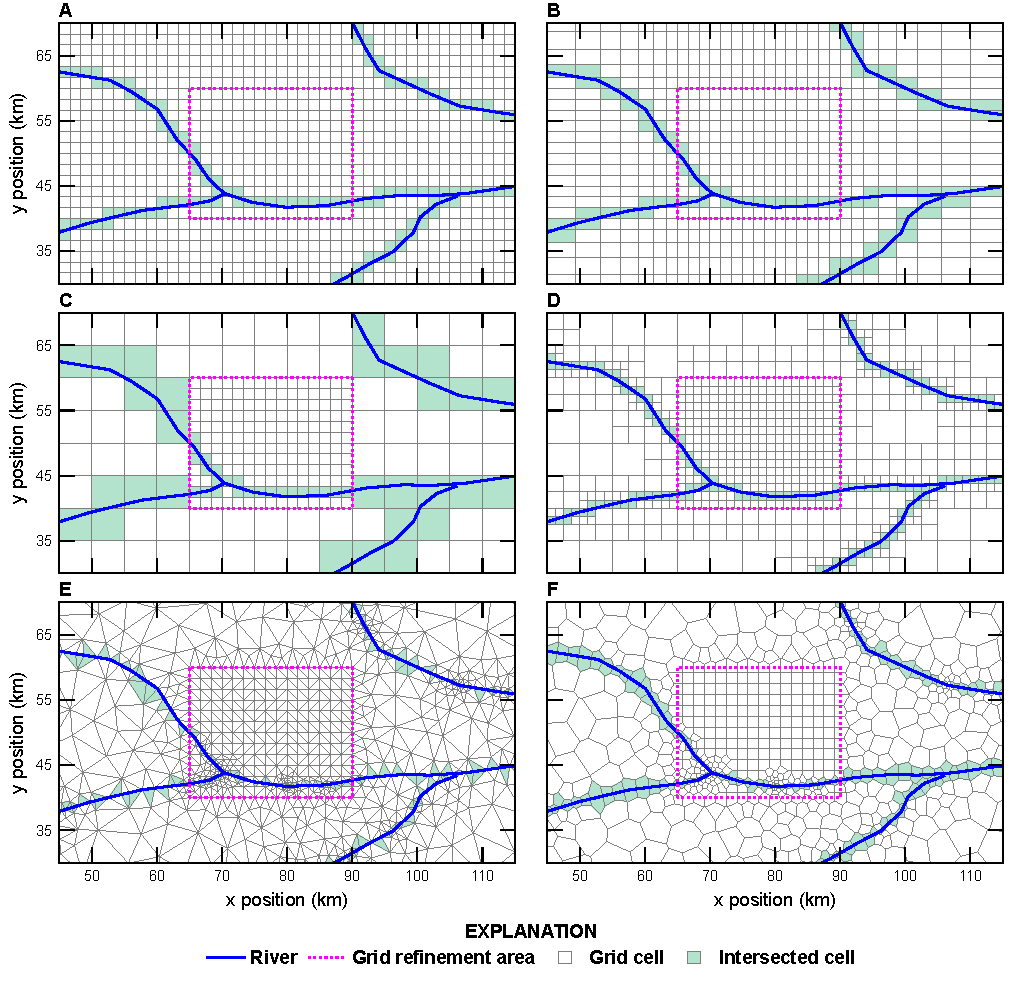
\includegraphics{figure2.pdf}
	\end{center}
	\caption{Examples of the intersection of a linear stream network with the model grids shown in Figure~\ref{fig:grids}. Intersections were performed using FloPy for (A) a structured MODFLOW grid, (B) a structured MODFLOW grid with variable row and column spacing, (C) a structured MODFLOW child grid nested within a structured MODFLOW parent grid, (D) a quadtree grid, (E) a triangular grid, and (F) a Voronoi grid. Shaded cells represent those cells that intersect with the linear stream network.}
	\label{fig:intersections}
\end{figure}


\subsection*{Processing MODFLOW 6 output}

MODFLOW 6 has many different types of output that can be created during a simulation. A GWF model, for example, can write simulated heads and detailed budget information to binary files. Global model budgets are written to standard MODFLOW listing (\texttt{*.lst}) files and can be written to comma-separated value text files. Some individual GWF and GWT model advanced stress packages can also write simulated output. Advanced packages solve their own continuity equation and include the Lake (LAK), Streamflow Routing (SFR), Multi-Aquifer Well (MAW), Unsaturated Zone Flow (UZF), and Mover (MVR) packages. For example, the LAK Package can write simulated lake stages and detailed lake budget information to binary files. Likewise, the MAW Package can write simulated well head and well budgets to binary files. Recent improvements have been made to FloPy to allow users easier access to simulation results using \texttt{.output} routines available for MODFLOW 6 models and advanced stress packages. Prior to these improvements, users were required to instantiate head, concentration, and budget file readers using file paths and names in order to access simulation results. With the \texttt{.output} routines, the file readers are automatically generated when called by the user.

The following \texttt{.methods()} syntax shows how a user can discover the type of output information that is available for the specified \texttt{gwf} model.

% not sure where there is a list() object here.
\begin{python}
>>> gwf.output.methods()
['list()', 'zonebudget()', 'budget()', 'budgetcsv()', 'head()']
\end{python}

\noindent The \texttt{.list()} method can be used to get the incremental (\texttt{incremental=True}) or cumulative budget information from the MODFLOW listing file for the \texttt{gwf} model for a user-specified simulation time, zero-based time step and stress period tuple, or zero-based index. The \texttt{.zonebudget()} method allows the user to build water and mass budgets for individual zones for MODFLOW 6 models, run the ZONEBUDGET program, and access ZONEBUDGET output. The \texttt{.budget()} method provides access to data in binary MODFLOW 6 cell-by-cell budget files. The \texttt{.budgetcsv()} method provides access to cumulative and incremental global budgets written by MODFLOW 6 to comma separated value files. The \texttt{.head()} method gives user access to data in the binary MODFLOW 6 head file.

Similarly, the following \texttt{.methods()} syntax shows how a user can discover the type of output information that is available for an advanced stress package, such as the LAK package.

\begin{python}
>>> gwf.lak.output.methods()
['zonebudget()', 'budget()', 'budgetcsv()', 'package_convergence()', 'obs()', 
 'stage()']
\end{python}

\noindent The \texttt{.package\_convergence()} method can be used to get the convergence information for an advanced stress package. The \texttt{.obs()} method can be used to get observation data saved for a model or stress package as a NumPy record array or pandas data frame. The \texttt{.stage()} method provides access to the dependent variable calculated by the LAK package and behaves similarly to the \texttt{.head()} method for the \texttt{gwf} model. 

\subsubsection*{Processing simulated dependent variables}

Simulated output for dependent variables are written by MODFLOW 6 to binary files. Simulated heads and concentrations written by the GWF and GWT models, respectively, can be accessed using the \texttt{.output} method on the FloPy \texttt{gwf} or \texttt{gwt} objects. To access the simulated head output, for example, a call can be made to the head file reader to retrieve data for a specified simulation time using the \texttt{.get\_data()} method as follows.

\begin{python}
head = gwf.output.head().get_data(totim=1.0)
\end{python}

\noindent In this case, the \texttt{head} variable is retrieved for a user-specified simulation time (\texttt{totim=} and is a NumPy array equal in size to the size of the model grid. Head data can also be accessed for a zero-based time step--stress period tuple

\begin{python}
head = gwf.output.head().get_data(kstpkper=(0,0))
\end{python}

\noindent or a zero-based index

\begin{python}
head = gwf.output.head().get_data(idx=0)
\end{python}

\subsubsection*{Processing simulated cell-by-cell budgets}

Similar to head output, cell-by-cell budget information can be accessed using FloPy. Unlike the simulated head file, the cell-by-cell budget file can have data for more than one item and these items may be stored in the file as arrays or lists of data. The data in the cell-by-cell budget file can be determined using

\begin{python}
>>> gwf.output.budget().list_unique_records()
RECORD           IMETH
----------------------
FLOW-JA-FACE         1
DATA-SPDIS           6
DATA-SAT             6
WEL                  6
DRN                  6
RCHA                 6
EVTA                 6
SFR                  6
LAK                  6
\end{python}

\noindent The \texttt{IMETH} code indicates if the data is stored in the file as an array (\texttt{IMETH=1}) or if it is list based (\texttt{IMETH=6}). Cell-by-cell specific-discharge data can be extracted using

\begin{python}
spdis = gwf.output.budget().get_data(totim=1.0, text="DATA-SPDIS")[0]
\end{python}

\noindent Simulated values for specific discharge for each cell are returned as a list containing a NumPy record array for the user-specified simulation time (\texttt{totim=}). Like MODFLOW head data, all of the data in the cell-by-cell data file for a user-specified simulation time (\texttt{totim=}), zero-based time step and stress period tuple (\texttt{kstpkper=}), or zero-based index (\texttt{idx=}) can also be extracted. Simulated specific discharge information can be processed into a form that can be plotted with FloPy using 

\begin{python}
qx, qy, qz = flopy.utils.postprocessing.get_specific_discharge(spdis, gwf, 
                                                               head=head)
\end{python}

\noindent The optional argument \texttt{head=} above sets the specific discharge in inactive or dry cells to a value that will not be plotted. 

\subsubsection*{Performing zone budget analyses}

\texttt{zonebudget()} output methods are available for both the \texttt{gwf} model and the \texttt{gwf.lak} advanced stress package examples shown above because they both solve a continuity equation. Other flow and transport advanced stress packages (\textit{e.g.}, SFR, Streamflow Transport (SFT), Unsaturated Zone Flow (UZF), Unsaturated Zone Transport (UZT), MAW, and Multi-Aquifer Well Transport (MWT)) also solve continuity equations and can be used with this zone budget functionality. The \texttt{zonebudget()} output method can be used to perform a zone budget analysis on the LAK advanced stress package using

\begin{python}
>>> zonbud = gwf.lak.output.zonebudget(zarr)
>>> zonbud.write_input()
>>> zonbud.run_model(silent=True)
(True, [])
\end{python}

\noindent \texttt{zarr} in the \texttt{gwf.lak.output.zonebudget()} is a NumPy array that defines an integer zone for each lake or group of lakes in the LAK advanced stress package. Zone budget output can be returned as a NumPy record array (\texttt{.get\_budget()} or \texttt{.get\_volumetric\_budget()}) or a pandas dataframe (\texttt{.get\_dataframes()}).

\subsection*{Plotting} \label{sec:plotting}

FloPy plotting capabilities have been refined and updated to support plotting both structured and unstructured models in map and cross-section view using the \texttt{.PlotMapView()} and \texttt{.PlotCrossSection()} classes, respectively. The plotting methods are wrappers around the Matplotlib plotting methods \citep{hunter2007matplotlib} and allow fine-grained control using Matplotlib keyword arguments (\texttt{kwargs}). The following Python code demonstrates the steps for plotting a map of simulated heads, the model grid, the location of drain (DRN) package cells, specific-discharge vectors, and head contours for the \texttt{gwf} model.

\begin{python}
mm = flopy.plot.PlotMapView(model=gwf)
mm.plot_array(head, edgecolor="0.5")
mm.plot_bc("DRN")
mm.plot_grid()
cs = mm.contour_array(head)
mm.ax.clabel(cs)
mm.plot_vector(qx, qy, normalize=True)
plt.show()
\end{python}

\noindent Figure~\ref{fig:flopyplots}A shows the outcome of the Python code demonstrated above with additional geographic features and fine-grained control of grid lines, text, annotations, tick locations, and axis labels. Results shown in Figure~\ref{fig:flopyplots} are for a steady-state model discretized into three convertible layers, with isotropic hydraulic properties, a hydraulic conductivity of 1 m/d, with rivers represented as drain cells in model in layer 1, and an areal recharge rate of 0.000001 m/d. Figure~\ref{fig:flopyplots}B shows use of the \texttt{.plot\_array()} method to create a map of the layer containing the water table, drain cells where the groundwater is discharging to a river, and cells where groundwater is discharging to the surface.

The following Python code demonstrates the steps for plotting a cross section of simulated heads and the model grid for the \texttt{gwf} model along an arbitrary line defined using a list of x, y coordinate pairs (tuples) defining the vertices of the line. For structured grids, cross sections can also be specified along a row or column.

\begin{python}
fx = flopy.plot.PlotCrossSection(model=gwf, 
                                 line={"line": [(0, 42500), (186801, 42500)]})
fx.plot_array(head, head=head)
fx.plot_grid()
plt.show()
\end{python}

\noindent The \texttt{head=} keyword option for the \texttt{plot\_array()} method above causes the plotting routine to draw and fill only the the saturated part of the model cell (determined using the simulated head and cell information). Without the \texttt{head=} keyword option, the entire cell from top to bottom would be color filled based on the head value. Figure~\ref{fig:flopyplots}C and D show the outcome of the Python code demonstrated along cross-section lines A--A' and B--B' (shown in Figure~\ref{fig:flopyplots}A) with additional fine-grained control of grid lines, text, annotations, tick locations, and axis labels. Note that the color flood of head in Figure~\ref{fig:flopyplots}C and D shows that unconfined conditions occur in higher elevation cells or cells adjacent to river cells.

\begin{figure}[ht!]
	\begin{center}
		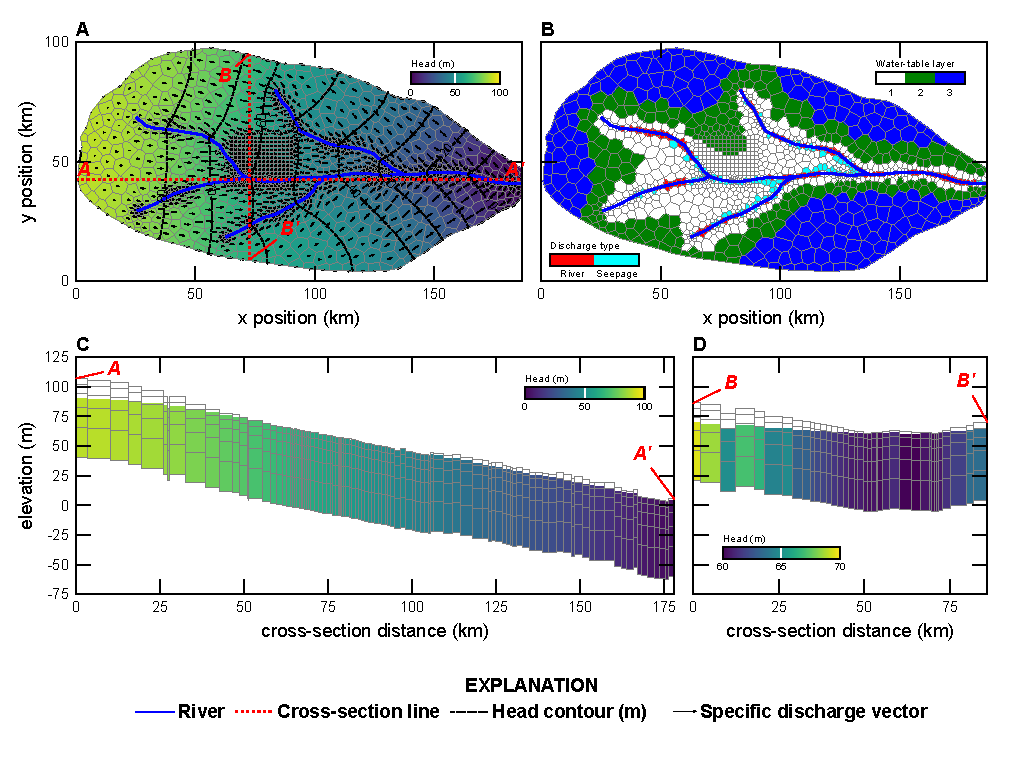
\includegraphics{figure3.pdf}
	\end{center}
	\caption{Examples of FloPy map and cross-section plotting capabilities for a model discretized using a Voronoi grid (Figure~\ref{fig:grids}F). (A) Map showing simulated heads and specific-discharge vectors in the upper-most saturated cells. (B) Map showing the layer containing the water table, the location of cells where the aquifer is discharged to rivers represented as drain cells, and the location of cells where groundwater is discharging to the land surface (seepage). (C) East-West cross-section along line A--A', shown on Figure~\ref{fig:flopyplots}A, showing the model grid, simulated heads, and cells where water-table conditions exist. (D) North-South cross-section along line B--B', shown on Figure~\ref{fig:flopyplots}A, showing the model grid, simulated heads, and cells where water-table conditions exist.}
	\label{fig:flopyplots}
\end{figure}

\subsection*{Exporting Grid Data to Other Formats}

Model input and output can be exported in a variety of standard formats using the \texttt{.export()} method, which is available for FloPy model objects, package objects, binary dependent-variable files (head, concentration, \textit{etc.}), and cell-by-cell output files. Standard output formats that are currently supported include shapefiles \citep{environmental1998esri}, NetCDF files \citep{rew2006netcdf, rew1990netcdf}, and Visualization Tool Kit (VTK) files \citep{schroeder:2006:VTK}. Entire models, packages, individual package arrays, binary dependent-variables (\textit{e.g.}, heads), or three-dimensional representations of binary cell-by-cell data can be exported. Shapefile and VTK output can be exported for all grid types, but currently, NetCDF output can only be exported for structured grids. The NetCDF output capability has been used to convert entire models and associated output so that it can be rendered in the GWWebFlow viewer \citep{gswebflow2018}.

The following Python code demonstrates the steps for exporting the \texttt{gwf} model as a VTK dataset with flat cell tops and bottoms (staircase representation).

\begin{python}
gwf.export("temp_vtk/vtk_staircase", fmt='vtk', smooth=False,
           vertical_exageration=500.0, pvd=True)
\end{python}

\noindent VTK models can also be exported with smooth cell tops and bottoms using elevations interpolated to the cell vertices (\texttt{smooth=True}). Other supported export formats can be created by specifying the file extension to be \texttt{.shp} for shapefiles, \texttt{.nc} for NetCDF files, or if the \texttt{fmt} keyword is \texttt{vtk} (as shown above) for VTK files. Figure~\ref{fig:flopyvtk} shows staircase and smooth VTK exports of the model described in the~\nameref{sec:plotting} section and rendered with ParaView \citep{ahrens2005paraview}.

\begin{figure}[ht!]
	\begin{center}
		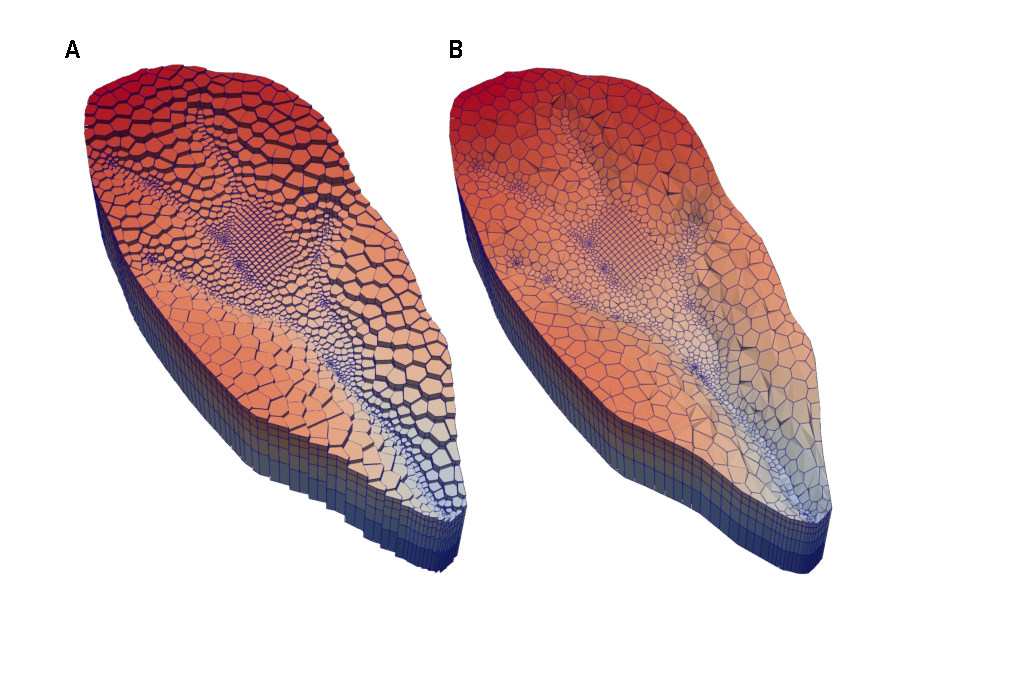
\includegraphics{figure4.pdf}
	\end{center}
	\caption{Two different graphical renderings of the Voronoi model grid: (A) staircase representation in which cell have flat tops and bottoms and (B) smooth representation in which elevations for cell vertices are interpolated using cell top and bottom elevations. Renderings were created using ParaView \citep{ahrens2005paraview} and Visualization Tool Kit \citep{schroeder:2006:VTK} files exported from FloPy.}
	\label{fig:flopyvtk}
\end{figure}

\section*{Scripting MODFLOW 6 Model Development Using Python and FloPy}

In this section, FloPy is used to construct, run, and post process a MODFLOW 6 model. All pre- and post-processing was done using FloPy grid, geospatial processing, MODFLOW 6 processing, and plotting functionality discussed previously. Figures~\ref{fig:mvgrid},~\ref{fig:mvmap},~\ref{fig:mvxsection}, and~\ref{fig:mvconc} were created using a combination of FloPy plotting functionality and Matplotlib plotting methods \citep{hunter2007matplotlib}. Jupyter notebooks \citep{Kluyver:2016aa} showing the commands for creating the model data sets, processing model results, and plotting these figures are available at the Synthetic Valley internet address indicated in the \nameref{sec:summary} section.

\cite{hill1998} present a synthetic test case (Synthetic Valley) of an undeveloped alluvial valley surrounded by low permeability bedrock. The model includes the Blue Lake and Straight River surface water features (Figure~\ref{fig:mvgrid}A). The model in \cite{hill1998} was calibrated and simulated using MODFLOWP \citep{hill1992computer} using a structured grid with a constant 152.4 m grid spacing, three model layers, and 1,000 active cells per layer. The upper two layers represent an unconfined aquifer, and the third layer represents a lower aquifer unit that is separated from the overlying aquifer by a confining unit in the northern part of the model domain (Figure~\ref{fig:mvgrid}A). The confining unit was not explicitly represented by \cite{hill1998}; instead a quasi-3D approach (low vertical conductance) between layers 2 and 3 was used to represent the confining unit.

%\lipsum[12-18]

\begin{figure}[ht!]
	\begin{center}
		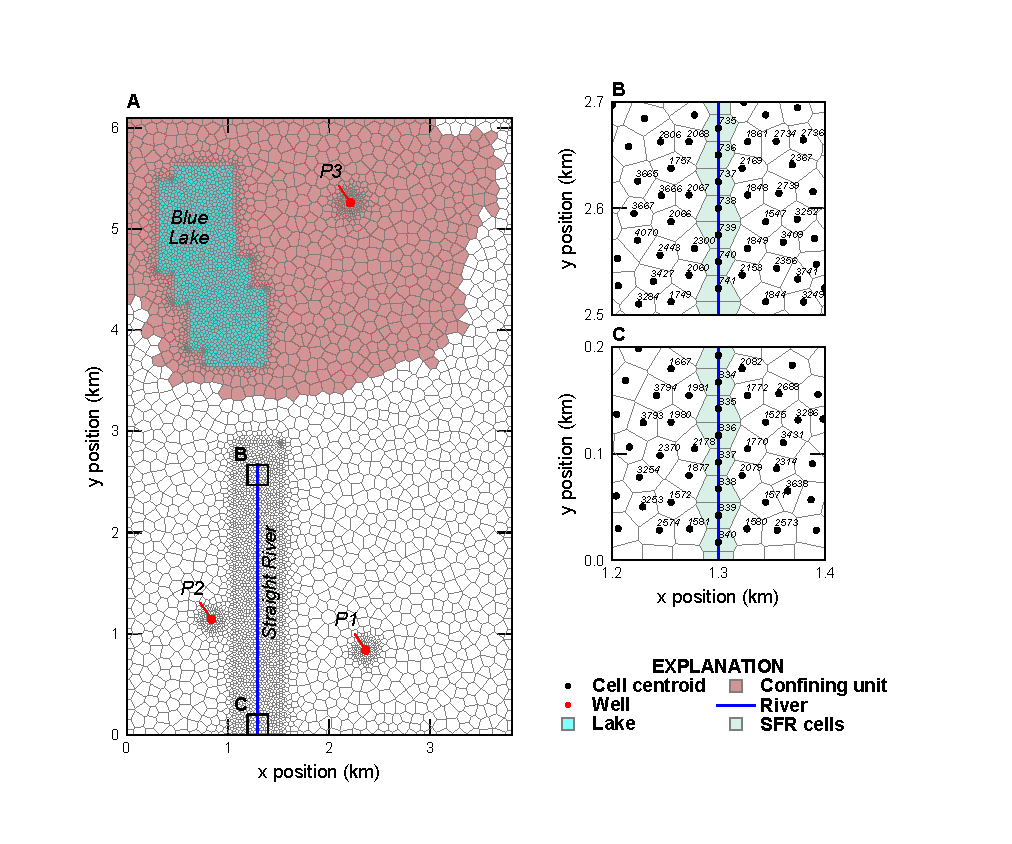
\includegraphics{figure5.pdf}
	\end{center}
	\caption{Synthetic Valley model used to demonstrate the MODFLOW 6 capabilities of FloPy. (A) Map showing the Voronoi grid used to discretize the model domain and the location of Blue Lake, Straight River, and the areal extent of the confining unit separating the upper and lower aquifer units. (B) Map showing model cells intersecting the northern end of Straight River. (C) Map showing model cells intersecting the southern end of Straight River. The cell centroid and cell numbers in the inset areas at the northern and southern end of Straight River are also shown on (B) and (C).}
	\label{fig:mvgrid}
\end{figure}

\subsection*{MODFLOW 6 Model Setup}

To demonstrate the capabilities of FloPy and MODFLOW 6, the 6,096 m x 3,810 m model domain is discretized using a Voronoi grid, with 6,343 active cells per layer, and the discretization by vertices (DISV) package (Figure~\ref{fig:mvgrid}A). The model grid was developed using the \texttt{Triangle()} and \texttt{VoronoiGrid()} utility classes. The model grid was refined within Blue Lake, around Straight River using a 750 m buffer, and around pumping wells P1, P2, and P3 using a 100 m buffer.

In this example, both groundwater flow \citep{modflow6gwf} and solute transport \citep{modflow6gwt} are simulated. To better represent solute transport, the lower aquifer has been discretized into three layers (instead of one). Confining units have to be explicitly simulated in MODFLOW 6, therefore, a total of six layers are simulated. The bottom of layers 1, 2, 3, and 4 were set to constant values of -1.53, -15.24, -15.55 and -30.48 m, respectively. Model layer 3 represents the confining unit and is relatively thin (0.3 m). The \texttt{IDOMAIN} concept \citep{modflow6gwf} was used to eliminate cells in model layer 3 (by setting \texttt{IDOMAIN=-1}) where the confining unit does not exist. In these areas, the thickness of layer 3 was set to zero and \texttt{IDOMAIN} was set to -1, which marks these cells in layer 3 as ``vertical pass through cells'' and results in cells in layer 2 being directly connected to cells in layer 4. 

The bottom of the model (layer 6) is based on \cite{hill1998} and the bottom of layer 5 was specified to be half the distance between the bottom of layers 4 and 6. The top of the model was constructed from topographic contours developed for the model that was used as the starting point for \cite{hill1998} \citep{pollock2014percomm}; the top of the model is shown in Figure~\ref{fig:mvmap}A. The top of the model and the bottom of layer 6 were resampled from the data used in the structured grid model using the \texttt{.resample\_to\_grid()} method available on the \texttt{VertexGrid} and linear interpolation. Figure~\ref{fig:mvxsection} shows the vertical discretization along cross-section lines A--A' and B--B', which are shown in Figure~\ref{fig:mvmap}A.

\begin{figure}[ht!]
	\begin{center}
		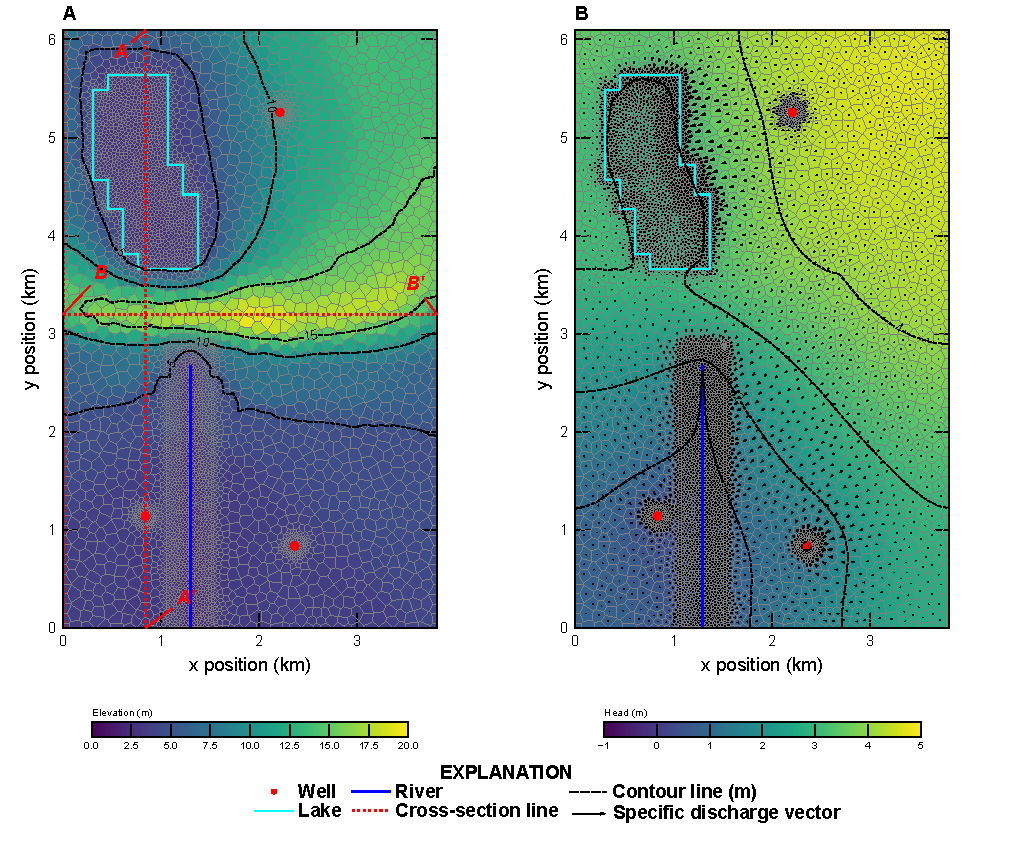
\includegraphics{figure6.pdf}
	\end{center}
	\caption{Map showing Synthetic Valley model (A) topography and (B) simulated steady-state heads and specific discharge rates in model layer 1. Cross-section lines A--A' and B--B' shown in Figure~\ref{fig:mvxsection} are also shown on (A).}
	\label{fig:mvmap}
\end{figure}

\begin{figure}[ht!]
	\begin{center}
		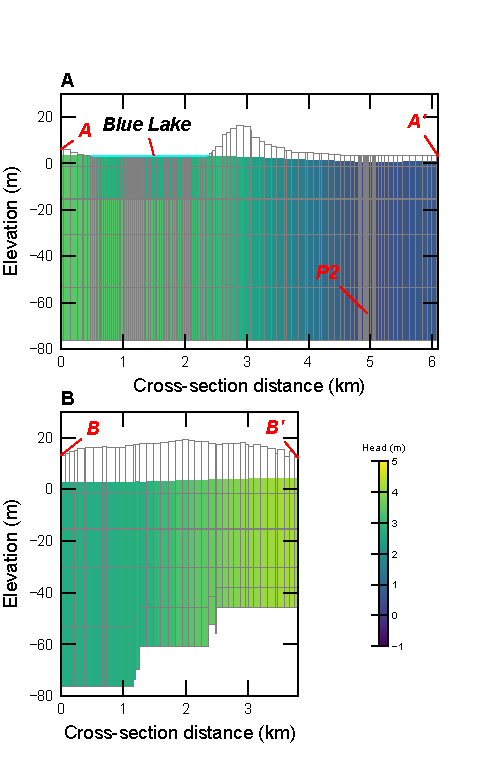
\includegraphics{figure7.pdf}
	\end{center}
	\caption{Cross-section of Synthetic Valley model grid and simulated steady-state heads along cross-section line (A) A--A' and (B) B--B'. The simulated Blue Lake steady-state stage (3.46 m) and pumping well P-2 are also shown on (A).}
	\label{fig:mvxsection}
\end{figure}

Hydraulic properties for the model were resampled from the data used in the structured grid model that was used as the starting point for \cite{hill1998} \citep{pollock2014percomm}. The horizontal hydraulic conductivity was discretized into five zones with values of 45.72, 50.29, 60.96, 83.82, and 121.92 m/d; the lowest hydraulic conductivity zone was located south of Blue Lake and the highest hydraulic conductivity zone was located beneath Blue Lake. The vertical hydraulic conductivity in the upper and lower aquifer was specified to be one quarter of the horizontal hydraulic conductivity. The horizontal and vertical hydraulic conductivity in the confining unit was set equal to 9.14$\times10^{-4}$ m/d. The horizontal and vertical hydraulic conductivity were resampled from the data used in the structured grid model using the \texttt{.resample\_to\_grid()} method on the \texttt{VertexGrid modelgrid} and the nearest neighbor algorithm.

For the groundwater transport model, the porosity was set to 0.2 in the upper and lower aquifer and 0.4 for cells in the confining unit. For the transport model, the Total Variation Diminishing scheme available in the GWT model \citep{modflow6gwt} was used to simulate advection. Dispersion was simulated using a longitudinal dispersivity of 75 m and a transverse dispersivity of 7.5 m. Molecular diffusion was not represented.

In the \cite{hill1998} representation of Synthetic Valley, the Straight River was simulated as head-dependent river (RIV) package cells, and Blue Lake was simulated as a high-hydraulic conductivity feature in model layer 1. In this recreation, Straight River is simulated using the streamflow routing (SFR) package, and Blue Lake is simulated using the LAK package. The SFR and LAK package cells were determined using \texttt{GridIntersect().intersect()} FloPy functionality (Figure~\ref{fig:mvgrid}A). 

Straight River was discretized into 108 SFR reaches. Cells that intersect the northern and southern end of Straight River are shown in Figures~\ref{fig:mvgrid}B and C. The bed thickness and width of each SFR reach was specified to be 0.3048 and 3.048 m, respectively. The leakance for each SFR reach was calculated using the bed thickness, reach width, and reach length in each cell and based on a total Straight River conductance of 50,971.72 m$^2$/d. A specified rainfall rate of 0.0025 m/d and a potential evaporation rate of 0.0019 m/d was defined for each Straight River reach.

Blue Lake was simulated as a lake on top of the model grid and only had vertical connections to 1,406 cells in the underlying upper aquifer (model layer 1). A bed leakance of 0.0013 1/d was specified for each cell connected to Blue Lake. A specified rainfall rate of 0.0025 m/d and a potential evaporation rate of 0.0019 m/d were defined for Blue Lake.

Drain (DRN) cells were specified in each cell in model layer 1 that was not connected to Blue Lake to prevent water levels from exceeding the top of the model. The conductance of each DRN cell was based on the horizontal cell area, a thickness of 0.3048 m, and a vertical hydraulic conductivity of 0.03048 m/d. Linear scaling of the drainage conductance was applied to improve model convergence and ranged from 0 m$^2$/d when groundwater levels were greater than or equal to 1 m below the top of the model to the specified conductance when groundwater water levels were greater than or equal to the top of the model.

Uniform recharge and potential evapotranspiration rates were specified using the recharge (RCH) and evapotranspiration (EVT) packages, respectively, and were equal to the rates specified in the SFR and LAK packages (0.0025 and 0.0019 m/d). The EVT surface was specified to be the top of the model and the EVT extinction depth was specified to be 1 m.

The location of pumping wells P1, P2, and P3 were determined using \texttt{GridIntersect().intersect()} FloPy functionality (Figure~\ref{fig:mvgrid}A). Pumping rates of -7,600, -7,600, and -1,900 m$^3$/d were specified for pumping wells P1, P2, and P3, respectively.

Transport was not simulated in the LAK and SFR packages. Instead, a specified concentration condition with a concentration of 1.0 mg/L was specified for Blue Lake. All other stress packages were assumed to have a concentration of 0 mg/L.

An initial head of 11 m was specified for every cell. An initial stage of 3.44 m was specified for Blue Lake. An initial concentration of 0 mg/L was specified for every cell in the transport model.

\subsection*{Simulated Results}
The groundwater flow model used the Newton-Raphson Formulation with Newton under-relaxation to improve convergence. The groundwater flow and transport models used the Bi-conjugate Stabilized (\texttt{bicgstab}) linear accelerator and \texttt{complexity="simple"} settings.
 
The groundwater flow and transport models were run for a total of 30 years. The groundwater flow model used a single steady-state time step and groundwater flow results were used to run the transport model with a total of 360 time steps with a constant length of 30.4375 days.
 
Simulated heads and vectors of specific discharge in model layer 1 are shown in Figure~\ref{fig:mvmap}B. Specific discharge is greatest on the east side of Blue Lake and in the vicinity of the three pumping wells and Straight River. Simulated heads along cross-sections A--A' and B--B' are shown in Figure~\ref{fig:mvxsection}. The cross sections show that water table conditions occur in most of the model domain except in the vicinity of Blue Lake.

Simulated concentrations at the end of 30-years in all six model layers are shown in Figure~\ref{fig:mvconc}. Simulated concentrations are highest beneath Blue Lake in model layer 1 and do not vary much in model layers 1 and 2. Simulated concentrations in model layer 3 are limited to the extent of the confining unit because the remaining cells in the layer are defined to be vertical pass through cells (\texttt{IDOMAIN=-1}). The lateral extent of the solute plume does not vary much south of Blue Lake because of the lack of confinement in these areas.

\begin{figure}[ht!]
	\begin{center}
		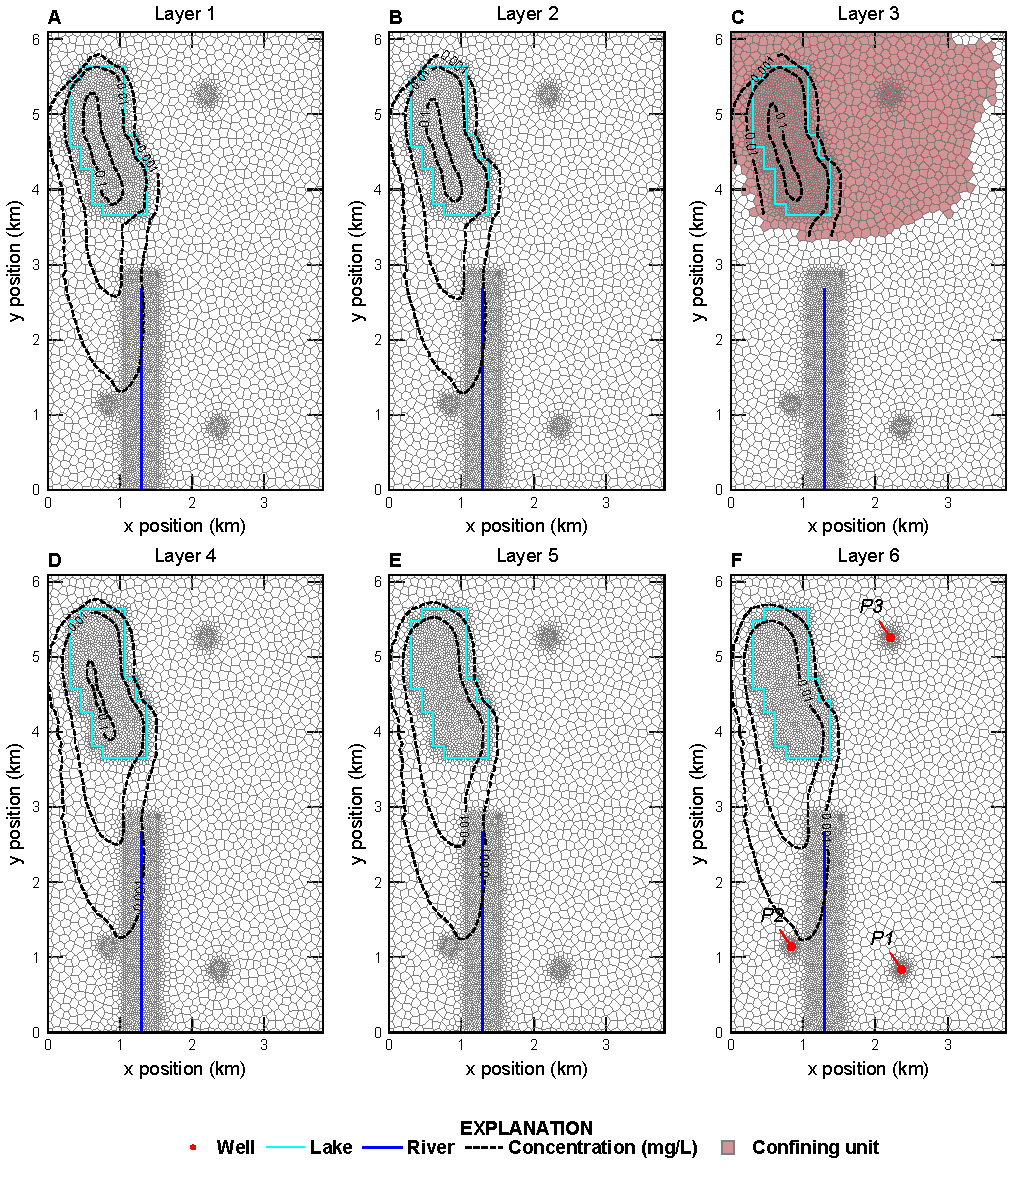
\includegraphics{figure8.pdf}
	\end{center}
	\caption{Maps showing Synthetic Valley simulated concentrations at the end of 30 years in model layer (A) 1, (B) 2, (C) 3, (D) 4, (E) 5, and (F) 6. The extent of the confining unit in model layer 3 is also shown on (C).}
	\label{fig:mvconc}
\end{figure}

\section*{Summary and Conclusions} \label{sec:summary}
FloPy is a Python package for building, running, and post processing groundwater models. It is open source and developed with input from a growing community of contributors. This paper summarizes new FloPy capabilities that have been added since the package was first described by \cite{bakker2016scripting}. The new and updated capabilities can be summarized as follows.

\begin{itemize}
\item FloPy supports the creation of many different types of groundwater models, including models that use MODFLOW 6, MODFLOW-2005, MODFLOW-NWT, MODFLOW-USG, MT3D, MT3D-USGS, and SEAWAT. FloPy support for MODFLOW 6 is based on an entirely new approach designed to automatically support all MODFLOW 6 models, packages, and options. The underlying FloPy classes for MODFLOW 6 are programmatically generated from the same input definition files that are used to construct the MODFLOW 6 user guide. This correspondence ensures that the FloPy classes are consistent and in-sync with MODFLOW 6 input.

\item FloPy has been extended to support unstructured model grids in addition to structured grids defined by layers, rows, and columns. FloPy has several different routines for creating unstructured grids. FloPy includes a wrapper for the GRIDGEN program \citep{gridgen}, which can be used to create layered quadtree grids. FloPy also includes a wrapper for the Triangle program \citep{trianglemesh}, which can be used to create triangular meshes. A triangular mesh can be converted by FloPy into a Voronoi grid. Grid information is stored for each FloPy model created by the user. This model grid object is used systemically throughout FloPy for geospatial operations, plotting, and exporting model information to supported formats.

\item Geospatial intersections of points, lines, and polygons with model grids and raster resampling onto model grids are common steps in model construction. FloPy fully supports these geospatial operations through its grid intersection and raster resampling routines.

\item Access to model output using FloPy has been simplified for MODFLOW 6 models. The new output access routines makes it possible to quickly extract simulated results from binary and text model output files.

\item FloPy supports plan-view map and cross-section plotting of model grids, boundary conditions, and simulated results. These plotting routines work with structured and unstructured models and can be customized to produce high quality figures.

\item FloPy supports the export of model information to shapefiles, VTK files, and NetCDF files. These exported files can then be loaded into other software programs, such as geographic information systems or advanced visualization programs for additional processing.

\end{itemize}

FloPy makes it possible to construct, and reproduce the construction, of a groundwater model from data in any format that can be accessed using Python. The robust new features in FloPy allow users to quickly try different model grids, different model spatial and temporal resolution, and different model configurations. 

The ability to script groundwater model construction and post-processing increases robustness, ensures reproducibility, provides a record of the data processing and model construction steps, and provides a means to improve the model and extend the simulation period as new data become available. The new geospatial processing routines make it possible to change model resolution as part of the model construction script. This allows one to prototype fast running models with coarse resolution and use finer resolution as the model starts to behave as intended. This workflow also allows one to conduct grid convergence studies to ensure that the grid is not the cause of unintended model behavior.

FloPy is open source and we welcome bug reports, code contributions, or improvements to the documentation from the community. The FloPy Python package can be installed using the \texttt{conda} or \texttt{pip} package managers. The source code, code documentation, tutorials, and examples can be found in the \href{https://github.com/modflowpy/flopy}{FloPy GitHub repository}. The Synthetic Valley example is available as a \href{https://modflow6-examples.readthedocs.io/en/master/examples.html}{MODFLOW 6 example} and the hypothetical watershed grid examples are available on the \href{https://github.com/modflowpy/flopy/tree/develop/examples/mf6_groundwater_paper}{FloPy GitHub repository}.

\section*{Acknowledgments}
The authors gratefully acknowledge the efforts of Mark Bakker and Vincent E.A. Post for initially developing FloPy and their continued efforts improving FloPy. Funding for this research was provided by the Enterprise Capacity project of the U.S. Geological Survey Integrated Water Prediction program.

\section*{Authors' Note}
The authors do not have any conflicts of interest to report.

\section*{Disclaimer}
Any use of trade, firm, or product names is for descriptive purposes only and does not imply endorsement by the U.S. Government.

\begin{thebibliography}{}

\bibitem[\protect\citeauthoryear{Ahrens, Geveci, and Law}{Ahrens
  et~al.}{2005}]{ahrens2005paraview}
Ahrens, J., B.~Geveci, and C.~Law. 2005.
\newblock ParaView: An End-User Tool for Large Data Visualization.
\newblock Visualization Handbook. Elsevier.

\bibitem[\protect\citeauthoryear{{{Australian Water School}}}{{{Australian
  Water School}}}{2023}]{auswat2023}
{{Australian Water School}}. 2023.
\newblock On-demand: {MODFLOW 6 and FloPy}.
\newblock \url{https://awschool.com.au/training/modflow6-flopy/} (accessed
  April 13, 2023).

\bibitem[\protect\citeauthoryear{Bakker, Post, Langevin, Hughes, White, Starn,
  and Fienen}{Bakker et~al.}{2016}]{bakker2016scripting}
Bakker, M., V.~Post, C.D. Langevin, J.D. Hughes, J.~White, J.~Starn, and M.N.
  Fienen. 2016.
\newblock {Scripting MODFLOW model development using Python and FloPy}.
\newblock {\em Groundwater\/}~54, no. 5: 733--739,
  \url{https://doi.org/10.1111/gwat.12413}.

\bibitem[\protect\citeauthoryear{Befus, Barnard, Hoover, Finzi~Hart, and
  Voss}{Befus et~al.}{2020}]{befus2020}
Befus, K.M., P.L. Barnard, D.J. Hoover, J.A. Finzi~Hart, and C.I. Voss. 2020.
\newblock {Increasing threat of coastal groundwater hazards from sea-level rise
  in California}.
\newblock {\em Nature Climate Change\/}~10, no. 10: 946--952,
  \url{https://doi.org/10.1038/s41558-020-0874-1}.

\bibitem[\protect\citeauthoryear{Befus, Kroeger, Smith, and Swarzenski}{Befus
  et~al.}{2017}]{befus2017}
Befus, K.M., K.D. Kroeger, C.G. Smith, and P.W. Swarzenski. 2017.
\newblock {The Magnitude and Origin of Groundwater Discharge to Eastern U.S.
  and Gulf of Mexico Coastal Waters}.
\newblock {\em Geophysical Research Letters\/}~44, no. 20: 10,396--10,406,
  \url{https://doi.org/10.1002/2017GL075238}.

\bibitem[\protect\citeauthoryear{Burek, Satoh, Kahil, Tang, Greve, Smilovic,
  Guillaumot, Zhao, and Wada}{Burek et~al.}{2020}]{burek2020}
Burek, P., Y.~Satoh, T.~Kahil, T.~Tang, P.~Greve, M.~Smilovic, L.~Guillaumot,
  F.~Zhao, and Y.~Wada. 2020.
\newblock {Development of the Community Water Model (CWatM v1.04) -- a
  high-resolution hydrological model for global and regional assessment of
  integrated water resources management}.
\newblock {\em Geoscientific Model Development\/}~13, no. 7: 3267--3298,
  \url{https://doi.org/10.5194/gmd-13-3267-2020}.

\bibitem[\protect\citeauthoryear{Ebeling, Handel, and Walther}{Ebeling
  et~al.}{2019}]{ebeling2019}
Ebeling, P., F.~Handel, and M.~Walther. 2019.
\newblock Potential of mixed hydraulic barriers to remediate seawater
  intrusion.
\newblock {\em Science of The Total Environment\/}~{\em 693}: 133478,
  \url{https://doi.org/10.1016/j.scitotenv.2019.07.284}.

\bibitem[\protect\citeauthoryear{Esri}{Esri}{1998}]{environmental1998esri}
Esri. 1998.
\newblock Esri Shapefile Technical Description, an ESRI white paper.
\newblock \url{http://www.esri.com/library/whitepapers/pdfs/shapefile.pdf}
  (accessed August 29, 2022).

\bibitem[\protect\citeauthoryear{Essawy, Goodall, Zell, Voce, Morsy, Sadler,
  Yuan, and Malik}{Essawy et~al.}{2018}]{essawy2018}
Essawy, B.T., J.L. Goodall, W.~Zell, D.~Voce, M.M. Morsy, J.~Sadler, Z.~Yuan,
  and T.~Malik. 2018.
\newblock {Integrating scientific cyberinfrastructures to improve
  reproducibility in computational hydrology: Example for HydroShare and
  GeoTrust}.
\newblock {\em Environmental Modelling \& Software\/}~{\em 105}: 217--229,
  \url{https://doi.org/10.1016/j.envsoft.2018.03.025}.

\bibitem[\protect\citeauthoryear{Fienen and Bakker}{Fienen and
  Bakker}{2016}]{fienen2016}
Fienen, M.N. and M.~Bakker. 2016.
\newblock HESS Opinions: Repeatable research: what hydrologists can learn from
  the Duke cancer research scandal.
\newblock {\em Hydrology and Earth System Sciences\/}~20, no. 9: 3739--3743,
  \url{https://doi.org/10.5194/hess-20-3739-2016}.

\bibitem[\protect\citeauthoryear{Fienen, Corson-Dosch, White, Leaf, and
  Hunt}{Fienen et~al.}{2022}]{fienen2022risk}
Fienen, M.N., N.T. Corson-Dosch, J.T. White, A.T. Leaf, and R.J. Hunt. 2022.
\newblock Risk-Based Wellhead Protection Decision Support: A Repeatable
  Workflow Approach.
\newblock {\em Groundwater\/}~60, no. 1: 71--86,
  \url{https://doi.org/10.3389/feart.2022.903965}.

\bibitem[\protect\citeauthoryear{Fienen, Haserodt, Leaf, and
  Westenbroek}{Fienen et~al.}{2022}]{fienen2022simulation}
Fienen, M.N., M.J. Haserodt, A.T. Leaf, and S.M. Westenbroek. 2022.
\newblock Simulation of regional groundwater flow and groundwater/lake
  interactions in the Central Sands, Wisconsin.
\newblock {U.S. Geological Survey Scientific Investigations Report 2022-5046,
  111 p.} \url{https://doi.org/10.3133/sir20225046}.

\bibitem[\protect\citeauthoryear{Gillies}{Gillies}{2022}]{shapely-gillies}
Gillies, S. 2022.
\newblock The shapely user manual.
\newblock \url{https://shapely.readthedocs.io/en/stable/manual.html} (accessed
  August 28, 2022).

\bibitem[\protect\citeauthoryear{Gillies et~al.}{Gillies
  et~al.}{2013}]{gillies_2019}
Gillies, S. et~al. 2013.
\newblock Rasterio: geospatial raster I/O for {Python} programmers.
\newblock \url{https://github.com/rasterio/rasterio} (accessed October 6,
  2022).

\bibitem[\protect\citeauthoryear{Guira}{Guira}{2018}]{Moussa2018}
Guira, M. 2018.
\newblock Numerical Modeling Of The Effects Of Land Use Change And Irrigation
  On Streamflow Depletion Of Frenchman Creek, Nebraska.
\newblock Master's thesis, University of Nebraska, Lincoln, NE.

\bibitem[\protect\citeauthoryear{{{Hatari Labs}}}{{{Hatari
  Labs}}}{2023}]{hatari2023}
{{Hatari Labs}}. 2023.
\newblock {Regional Groundwater Modeling with MODFLOW and Flopy - Tutorial}.
\newblock
  \url{https://hatarilabs.com/ih-en/regional-groundwater-modeling-with-modflow-and-flopy-tutorial}
  (accessed April 13, 2023).

\bibitem[\protect\citeauthoryear{Hill}{Hill}{1992}]{hill1992computer}
Hill, M.C. 1992.
\newblock A computer program (MODFLOWP) for estimating parameters of a
  transient, three-dimensional, ground-water flow model using nonlinear
  regression.
\newblock {U.S. Geological Survey Open-File Report 91-484, 358 p.}

\bibitem[\protect\citeauthoryear{Hill, Cooley, and Pollock}{Hill
  et~al.}{1998}]{hill1998}
Hill, M.C., R.L. Cooley, and D.W. Pollock. 1998.
\newblock A Controlled Experiment in Ground Water Flow Model Calibration.
\newblock {\em Groundwater\/}~36, no. 3: 520--535,
  \url{https://doi.org/10.1111/j.1745-6584.1998.tb02824.x}.

\bibitem[\protect\citeauthoryear{Hughes, Langevin, and Banta}{Hughes
  et~al.}{2017}]{modflow6framework}
Hughes, J.D., C.D. Langevin, and E.R. Banta. 2017.
\newblock Documentation for the MODFLOW 6 framework.
\newblock {U.S. Geological Survey Techniques and Methods, book 6, chap. A57, 36
  p.} \url{https://doi.org/10.3133/tm6A57}.

\bibitem[\protect\citeauthoryear{Hughes, Leake, Galloway, and White}{Hughes
  et~al.}{2022}]{modflow6csub}
Hughes, J.D., S.A. Leake, D.L. Galloway, and J.W. White. 2022.
\newblock Documentation for the Skeletal Storage, Compaction, and Subsidence
  (CSUB) Package of MODFLOW 6.
\newblock {U.S. Geological Survey Techniques and Methods, book 6, chap. A62, 57
  p.} \url{https://doi.org/10.3133/tm6A62}.

\bibitem[\protect\citeauthoryear{Hunter}{Hunter}{2007}]{hunter2007matplotlib}
Hunter, J.D. 2007.
\newblock Matplotlib: A 2D graphics environment.
\newblock {\em Computing in science \& engineering\/}~9, no. 03: 90--95.

\bibitem[\protect\citeauthoryear{Jaxa-Rozen, Kwakkel, and
  Bloemendal}{Jaxa-Rozen et~al.}{2019}]{jaxarozen2019}
Jaxa-Rozen, M., J.H. Kwakkel, and M.~Bloemendal. 2019.
\newblock A coupled simulation architecture for agent-based/geohydrological
  modelling with NetLogo and MODFLOW.
\newblock {\em Environmental Modelling \& Software\/}~{\em 115}: 19--37,
  \url{https://doi.org/10.1016/j.envsoft.2019.01.020}.

\bibitem[\protect\citeauthoryear{Kluyver, Ragan-Kelley, P{\'e}rez, Granger,
  Bussonnier, Frederic, Kelley, Hamrick, Grout, Corlay, Ivanov, Avila, Abdalla,
  and Willing}{Kluyver et~al.}{2016}]{Kluyver:2016aa}
Kluyver, T., B.~Ragan-Kelley, F.~P{\'e}rez, B.~Granger, M.~Bussonnier,
  J.~Frederic, K.~Kelley, J.~Hamrick, J.~Grout, S.~Corlay, P.~Ivanov, D.~Avila,
  S.~Abdalla, and C.~Willing. 2016.
\newblock Jupyter Notebooks -- a publishing format for reproducible
  computational workflows.
\newblock In F.~Loizides and B.~Schmidt (Eds.), {\em Positioning and Power in
  Academic Publishing: Players, Agents and Agendas}, pp.\  87 -- 90. IOS Press,
  \url{https://doi.org/10.3233/978-1-61499-649-1-87}.

\bibitem[\protect\citeauthoryear{Knowling, White, and Moore}{Knowling
  et~al.}{2019}]{knowling2019}
Knowling, M.J., J.T. White, and C.R. Moore. 2019.
\newblock Role of model parameterization in risk-based decision support: An
  empirical exploration.
\newblock {\em Advances in Water Resources\/}~{\em 128}: 59--73,
  \url{https://doi.org/10.1016/j.advwatres.2019.04.010}.

\bibitem[\protect\citeauthoryear{Langevin, Hughes, Provost, Banta, Niswonger,
  and Panday}{Langevin et~al.}{2017}]{modflow6gwf}
Langevin, C.D., J.D. Hughes, A.M. Provost, E.R. Banta, R.G. Niswonger, and
  S.~Panday. 2017.
\newblock Documentation for the MODFLOW 6 Groundwater Flow (GWF) Model.
\newblock {U.S. Geological Survey Techniques and Methods, book 6, chap. A55,
  197 p.} \url{https://doi.org/10.3133/tm6A55}.

\bibitem[\protect\citeauthoryear{Langevin, Panday, and Provost}{Langevin
  et~al.}{2020}]{langevin2020hydraulic}
Langevin, C.D., S.~Panday, and A.M. Provost. 2020.
\newblock Hydraulic-Head Formulation for Density-Dependent Flow and Transport.
\newblock {\em Groundwater\/}~58, no. 3: 349--362.

\bibitem[\protect\citeauthoryear{Langevin, Provost, Panday, and
  Hughes}{Langevin et~al.}{2022}]{modflow6gwt}
Langevin, C.D., A.M. Provost, S.~Panday, and J.D. Hughes. 2022.
\newblock Documentation for the MODFLOW 6 Groundwater Transport (GWT) Model.
\newblock {U.S. Geological Survey Techniques and Methods, book 6, chap. A61, 56
  p.} \url{https://doi.org/10.3133/tm6A55}.

\bibitem[\protect\citeauthoryear{Larsen, Alzraiee, Martin, and
  Niswonger}{Larsen et~al.}{2022}]{larsen2022rapid}
Larsen, J.D., A.H. Alzraiee, D.~Martin, and R.G. Niswonger. 2022.
\newblock Rapid Model Development for GSFLOW With Python and pyGSFLOW.
\newblock {\em Frontiers in Earth Science\/}~{\em 10},
  \url{https://doi.org/10.3389/feart.2022.907533}.

\bibitem[\protect\citeauthoryear{Leaf and Fienen}{Leaf and
  Fienen}{2022}]{leaf2022modflow}
Leaf, A.T. and M.N. Fienen. 2022.
\newblock Modflow-setup: Robust automation of groundwater model construction.
\newblock {\em Frontiers in Earth Science\/}~{\em 10}: 903965,
  \url{https://doi.org/10.3389/feart.2022.903965}.

\bibitem[\protect\citeauthoryear{Lien, Liu, and Langevin}{Lien
  et~al.}{2014}]{gridgen}
Lien, J.M., G.~Liu, and C.D. Langevin. 2014.
\newblock GRIDGEN Version 1.0: A computer program for generating unstructured
  finite-volume grids.
\newblock {U.S. Geological Survey Open-File Report 2014--1109, 26 p.}
  \url{https://doi.org/10.3133/ofr20141109}.

\bibitem[\protect\citeauthoryear{Mancewicz, Mayer, Langevin, and
  Gulley}{Mancewicz et~al.}{2022}]{modflow6lkt}
Mancewicz, L.K., A.~Mayer, C.D. Langevin, and J.~Gulley. 2022.
\newblock Improved method for simulating groundwater inundation using the
  MODFLOW 6 Lake Transport Package.
\newblock {\em Groundwater\/}, \url{https://doi.org/10.1111/gwat.13254}.

\bibitem[\protect\citeauthoryear{Mehl and Hill}{Mehl and
  Hill}{2006}]{modflowlgr}
Mehl, S.W. and M.C. Hill. 2006.
\newblock {MODFLOW-2005, the U.S. Geological Survey modular ground-water
  model-documentation of shared node local grid refinement (LGR) and the
  boundary flow and head (BFH) package}.
\newblock {U.S. Geological Survey Techniques and Methods, book 6, chap. A12, 78
  p.} \url{https://doi.org/10.3133/tm6A12}.

\bibitem[\protect\citeauthoryear{Mehl and Hill}{Mehl and
  Hill}{2013}]{modflowlgr2}
Mehl, S.W. and M.C. Hill. 2013.
\newblock MODFLOW-LGR---Documentation of ghost node local grid refinement
  (LGR2) for multiple areas and the boundary flow and head (BFH2) package.
\newblock {U.S. Geological Survey Techniques and Methods, book 6, chap. A44, 43
  p.} \url{https://doi.org/10.3133/tm6A44}.

\bibitem[\protect\citeauthoryear{Morway, Langevin, and Hughes}{Morway
  et~al.}{2021}]{morway2021use}
Morway, E.D., C.D. Langevin, and J.D. Hughes. 2021.
\newblock Use of the {MODFLOW 6} water mover package to represent natural and
  managed hydrologic connections.
\newblock {\em Groundwater\/}~59, no. 6: 913--924,
  \url{https://doi.org/10.1111/gwat.13117}.

\bibitem[\protect\citeauthoryear{Panday, Langevin, Niswonger, Ibaraki, and
  Hughes}{Panday et~al.}{2013}]{modflowusg}
Panday, S., C.D. Langevin, R.G. Niswonger, M.~Ibaraki, and J.D. Hughes. 2013.
\newblock MODFLOW-USG version 1---An unstructured grid version of MODFLOW for
  simulating groundwater flow and tightly coupled processes using a control
  volume finite-difference formulation.
\newblock {U.S. Geological Survey Techniques and Methods, book 6, chap. A45, 66
  p.}

\bibitem[\protect\citeauthoryear{Perry}{Perry}{2013}]{perry2013}
Perry, M. 2013.
\newblock Rasterstats python library.
\newblock \url{https://github.com/perrygeo/python-rasterstats}.

\bibitem[\protect\citeauthoryear{Pollock}{Pollock}{2014}]{pollock2014percomm}
Pollock, D.W. 2014.
\newblock Personal communication.
\newblock Reston, VA.

\bibitem[\protect\citeauthoryear{Provost, Langevin, and Hughes}{Provost
  et~al.}{2017}]{modflow6xt3d}
Provost, A.M., C.D. Langevin, and J.D. Hughes. 2017.
\newblock Documentation for the ``XT3D'' Option in the Node Property Flow (NPF)
  Package of MODFLOW 6.
\newblock {U.S. Geological Survey Techniques and Methods, book 6, chap. A56, 46
  p.} \url{https://doi.org/10.3133/tm6A56}.

\bibitem[\protect\citeauthoryear{Rew and Davis}{Rew and
  Davis}{1990}]{rew1990netcdf}
Rew, R. and G.~Davis. 1990.
\newblock NetCDF: an interface for scientific data access.
\newblock {\em IEEE computer graphics and applications\/}~10, no. 4: 76--82.

\bibitem[\protect\citeauthoryear{Rew, Hartnett, Caron, et~al.}{Rew
  et~al.}{2006}]{rew2006netcdf}
Rew, R., E.~Hartnett, J.~Caron, et~al. 2006.
\newblock NetCDF-4: Software implementing an enhanced data model for the
  geosciences.
\newblock In {\em 22nd International Conference on Interactive Information
  Processing Systems for Meteorology, Oceanograph, and Hydrology}, Volume~6.

\bibitem[\protect\citeauthoryear{Rossetto, {De Filippis}, Borsi, Foglia,
  Cannata, Criollo, and V{\'a}zquez-Su{\~n}{\'e}}{Rossetto
  et~al.}{2018}]{freewat2018}
Rossetto, R., G.~{De Filippis}, I.~Borsi, L.~Foglia, M.~Cannata, R.~Criollo,
  and E.~V{\'a}zquez-Su{\~n}{\'e}. 2018.
\newblock Integrating free and open source tools and distributed modelling
  codes in {GIS} environment for data-based groundwater management.
\newblock {\em Environmental Modelling \& Software\/}~{\em 107}: 210--230,
  \url{https://doi.org/10.1016/j.envsoft.2018.06.007}.

\bibitem[\protect\citeauthoryear{Schroeder, Martin, and Lorensen}{Schroeder
  et~al.}{2006}]{schroeder:2006:VTK}
Schroeder, W., K.~Martin, and B.~Lorensen. 2006.
\newblock {\em The Visualization Toolkit\/} (4th ed.).
\newblock Kitware.

\bibitem[\protect\citeauthoryear{Shewchuk}{Shewchuk}{1996}]{trianglemesh}
Shewchuk, J.R. 1996.
\newblock Triangle: Engineering a {2D} Quality Mesh Generator and Delaunay
  Triangulator.
\newblock In {\em Applied Computational Geometry, Towards Geometric
  Engineering, FCRC'96 Workshop, WACG'96, Philadelphia, PA, USA, May 27-28,
  1996, Selected Papers}, pp.\  203--222.
  \url{https://doi.org/10.1007/BFb0014497}.

\bibitem[\protect\citeauthoryear{Starn and Belitz}{Starn and
  Belitz}{2018}]{starn2018}
Starn, J.J. and K.~Belitz. 2018.
\newblock Regionalization of Groundwater Residence Time Using Metamodeling.
\newblock {\em Water Resources Research\/}~54, no. 9: 6357--6373,
  \url{https://doi.org/10.1029/2017WR021531}.

\bibitem[\protect\citeauthoryear{Sun}{Sun}{2018}]{sun2018}
Sun, A.Y. 2018.
\newblock Discovering State-Parameter Mappings in Subsurface Models Using
  Generative Adversarial Networks.
\newblock {\em Geophysical Research Letters\/}~45, no. 20: 11,137--11,146,
  \url{https://doi.org/10.1029/2018GL080404}.

\bibitem[\protect\citeauthoryear{{U.S. Geological Survey}}{{U.S. Geological
  Survey}}{2018}]{gswebflow2018}
{U.S. Geological Survey}. 2018.
\newblock GWWebFlow--a browser-based groundwater model viewer.
\newblock \url{https://webapps.usgs.gov/gwwebflow/}.

\bibitem[\protect\citeauthoryear{{van Engelen}, {Oude Essink}, Kooi, and
  Bierkens}{{van Engelen} et~al.}{2018}]{vanengelen2018}
{van Engelen}, J., G.H. {Oude Essink}, H.~Kooi, and M.F. Bierkens. 2018.
\newblock On the origins of hypersaline groundwater in the {Nile Delta}
  aquifer.
\newblock {\em Journal of Hydrology\/}~{\em 560}: 301--317,
  \url{https://doi.org/10.1016/j.jhydrol.2018.03.029}.

\bibitem[\protect\citeauthoryear{Vilhelmsen, Christensen, and Mehl}{Vilhelmsen
  et~al.}{2012}]{vilhelmsen2012evaluation}
Vilhelmsen, T.N., S.~Christensen, and S.W. Mehl. 2012.
\newblock Evaluation of MODFLOW-LGR in connection with a synthetic
  regional-scale model.
\newblock {\em Groundwater\/}~50, no. 1: 118--132,
  \url{https://doi.org/10.1111/j.1745-6584.2011.00826.x}.

\bibitem[\protect\citeauthoryear{Virtanen, Gommers, Oliphant, Haberland, Reddy,
  Cournapeau, Burovski, Peterson, Weckesser, Bright, {van der Walt}, Brett,
  Wilson, Millman, Mayorov, Nelson, Jones, Kern, Larson, Carey, Polat, Feng,
  Moore, {VanderPlas}, Laxalde, Perktold, Cimrman, Henriksen, Quintero, Harris,
  Archibald, Ribeiro, Pedregosa, {van Mulbregt}, and {SciPy 1.0
  Contributors}}{Virtanen et~al.}{2020}]{2020SciPy-NMeth}
Virtanen, P., R.~Gommers, T.E. Oliphant, M.~Haberland, T.~Reddy, D.~Cournapeau,
  E.~Burovski, P.~Peterson, W.~Weckesser, J.~Bright, S.J. {van der Walt},
  M.~Brett, J.~Wilson, K.J. Millman, N.~Mayorov, A.R.J. Nelson, E.~Jones,
  R.~Kern, E.~Larson, C.J. Carey, {\.I}.~Polat, Y.~Feng, E.W. Moore,
  J.~{VanderPlas}, D.~Laxalde, J.~Perktold, R.~Cimrman, I.~Henriksen, E.A.
  Quintero, C.R. Harris, A.M. Archibald, A.H. Ribeiro, F.~Pedregosa, P.~{van
  Mulbregt}, and {SciPy 1.0 Contributors}. 2020.
\newblock {{SciPy} 1.0: Fundamental Algorithms for Scientific Computing in
  Python}.
\newblock {\em Nature Methods\/}~{\em 17}: 261--272,
  \url{https://doi.org/10.1038/s41592-019-0686-2}.

\bibitem[\protect\citeauthoryear{White}{White}{2018}]{white2018ies}
White, J.T. 2018.
\newblock A model-independent iterative ensemble smoother for efficient
  history-matching and uncertainty quantification in very high dimensions.
\newblock {\em Environmental Modelling \& Software\/}~{\em 109}: 191--201,
  \url{https://doi.org/10.1016/j.envsoft.2018.06.009}.

\bibitem[\protect\citeauthoryear{White, Foster, Fienen, Knowling, Hemmings, and
  Winterle}{White et~al.}{2020}]{white2020toward}
White, J.T., L.K. Foster, M.N. Fienen, M.J. Knowling, B.~Hemmings, and J.R.
  Winterle. 2020.
\newblock Toward reproducible environmental modeling for decision support: A
  worked example.
\newblock {\em Frontiers in Earth Science\/}~{\em 8}: 50,
  \url{https://doi.org/10.3389/feart.2020.00050}.

\bibitem[\protect\citeauthoryear{Zhou and Tartakovsky}{Zhou and
  Tartakovsky}{2021}]{zhou2021}
Zhou, Z. and D.M. Tartakovsky. 2021.
\newblock Markov chain Monte Carlo with neural network surrogates: application
  to contaminant source identification.
\newblock {\em Stochastic Environmental Research and Risk Assessment\/}~35, no.
  10: 639--651, \url{https://doi.org/10.1007/s00477-020-01888-9}.

\bibitem[\protect\citeauthoryear{Zipper, Gleeson, Kerr, Howard, Rohde, Carah,
  and Zimmerman}{Zipper et~al.}{2019}]{zipper2019}
Zipper, S.C., T.~Gleeson, B.~Kerr, J.K. Howard, M.M. Rohde, J.~Carah, and
  J.~Zimmerman. 2019.
\newblock Rapid and Accurate Estimates of Streamflow Depletion Caused by
  Groundwater Pumping Using Analytical Depletion Functions.
\newblock {\em Water Resources Research\/}~55, no. 7: 5807--5829,
  \url{https://doi.org/10.1029/2018WR024403}.

\end{thebibliography}

\begingroup
	\hyphenpenalty10000
	\renewcommand{\listfigurename}{Figure captions}
	\listoffigures
\endgroup

\end{document}
